% JKAIA 2026 (2026 한국인공지능학회 추계학술대회) -- General (Poster) 트랙, 한국어 작업본
% ※ 제출본은 영문 main.tex다. 이 파일은 저자가 내용을 검토·수정하기 위한 한국어 대조본이며, 문단 구조가 main.tex와 1:1로 같다.
%    이 파일을 고치면 같은 자리의 영문을 main.tex에 반영한다. 한국어판은 쪽수 제한(2쪽)을 지키지 않아도 된다.
% 템플릿: kaia.cls (포스터 트랙 공식 zip, 2026-10 배포본, 10pt, A4). 2026-10-24에 다시 받아 바이트 단위로 같음을 확인했다.
% 심사는 single-blind이므로 저자를 명기한다.
%
% 학회 논문제출 안내(2026-10-24 확인): "제출 논문은 영문으로 작성", 이지체어에는 제목 영문·초록 국문 → 영문 main.tex를 제출한다.
% 템플릿 초록 규칙: 10~20줄, 제목과 초록에 기호·특수문자·각주·수식을 쓰지 않는다.
%
% 빌드: tectonic -X compile main_ko.tex  (XeTeX: 한글은 kotex/xetexko + Apple SD Gothic Neo)
%
% 템플릿 대비 변경점(main.tex와 같음):
%  * 템플릿의 \fbox{\parbox}는 쪽을 넘기지 못하므로 두 쪽 요약을 위해 mdframed로 같은 테두리를 그린다.
%  * kaia.cls의 \maketitle이 \twocolumn[...]을 호출하므로 \twocolumn을 1단으로 재정의해 템플릿 PDF와 같은 1단을 유지한다.
%  * XeTeX에서는 Times(mathptmx)가 매핑되지 않아 시스템 Times New Roman을 쓴다.

\documentclass[nouppercase]{kaia}
\usepackage{amsmath}
\usepackage{booktabs}
\usepackage{graphicx}
\usepackage[framemethod=TikZ]{mdframed}
\usepackage{iftex}
\ifXeTeX
  \usepackage{fontspec}
  \setmainfont{Times New Roman}
  \usepackage{kotex}
  \setmainhangulfont{Apple SD Gothic Neo}[BoldFont={* Bold}, ItalicFont={* Light}]
\else
  \usepackage{kotex}
\fi
\graphicspath{{../figures/}}

\makeatletter
\renewcommand{\twocolumn}[1][]{#1}   % 1단 유지; \maketitle의 선택 인자는 그대로 조판된다
\@secpenalty=0   % mdframed 안에서 음수 절 penalty가 C절 앞에서 틀을 끊어 1쪽이 짧아지던 문제
\makeatother
\mdfsetup{linewidth=0.4pt, linecolor=black, innerleftmargin=7pt, innerrightmargin=7pt,
          innertopmargin=3pt, innerbottommargin=2pt, skipabove=1pt, skipbelow=1pt}

\title{Near-Miss Blindness: latent 월드모델의 상상은 결과 경계의 해상도를 잃는다\\[2pt]
{\normalsize\normalfont Near-Miss Blindness: Latent World-Model Imagination Loses Resolution at the Outcome Boundary}}

\author{송용휘}{a}
\author{이건명}{b}
\affiliation{충북대학교 정보통신공학부, 대한민국, thddydgnl1937@gmail.com}{a}
\affiliation{충북대학교 소프트웨어학부, 대한민국, kmlee@cbnu.ac.kr}{b}

\begin{document}

\maketitle
\vspace{-34pt}

\begin{mdframed}

\begin{abstract}
로봇 정책 평가에 쓰이는 학습된 월드모델은 실패한 실행을 성공으로 상상한다고 보고되어 왔다. 본 연구는 어떤 실패가 오판되는지를 묻는다. 성공 경계 주변에 반사실 실패를 촘촘하게 만들어 실패 거리(과제 오차를 성공 문턱으로 나눈 값)로 정렬하고, 실제 최종 프레임과 상상 최종 프레임을 같은 판정기로 판정해 판정기 자체의 오차와 상상이 더한 오차를 분리한다. 가설, 문턱, 판정 규칙은 시각과 해시를 기록한 내부 설계 문서로 사전등록했다. 공개 DINO-WM PushT 모델에서 상상 길이가 5단계일 때 상상은 성공과 먼 실패를 여전히 구분하지만 경계의 해상도는 잃는다. 성공 대 near-miss AUROC는 실제 프레임의 0.953에서 상상의 0.853으로 떨어지는 반면 성공 대 far-miss AUROC는 0.005만 떨어지며, near-miss 쪽 하락은 상상 길이와 함께 커진다. 상상 특징으로 학습한 판별기도 0.889에 그쳐 경계 정보의 일부가 사라지며, 오판은 낙관 쪽이 아니라 양방향으로 일어난다. 통제된 latent 모델에서 학습 데이터의 실패율을 0.3에서 0.03으로 낮추면 near-miss를 성공으로 상상하는 비율이 0.10에서 0.54로 늘고 이 오판은 모두 상상에서 생기며, 성공을 실패로 보는 오판은 0으로 줄어든다. 공개 모델에서 재학습 없는 MC dropout 할인의 효과는 작았고, 두 latent 모델 모두에서 경계를 겨냥한 반사실 데이터는 단순 재가중보다 낫지 않았다. 비디오 월드모델에서는 사전등록한 경계 특이성 가설이 지지되지 않아, 주장의 범위를 시험한 두 latent 모델로 한정한다.
\end{abstract}
\begin{keywords}
World models, robot policy evaluation, failure prediction, imagination, pre-registration
\end{keywords}

\subsection{Problem Setup (문제 설정)}
DINO-WM~[1] 같은 latent 계획 모델부터 Cosmos Policy~[2] 같은 비디오 정책 모델까지, 월드모델은 로봇 정책을 상상 속에서 평가할 수 있다. 실제 초기 관측에서 정책의 행동을 월드모델로 굴리고, 성공 판정기가 상상된 최종 프레임을 판정한다. 상상이 실패한 실행을 성공으로 예측한다는 보고가 있다~[3, 4]. 본 연구는 이 오판이 실패가 경계에서 얼마나 먼지에 따라 어떻게 달라지는지 묻는다. 실패 거리는 $r=e/\tau$, 즉 과제 오차를 성공 문턱으로 나눈 값이다(성공 $r<1$, near-miss $1\le r<2$, far-miss $r\ge 3$). 측정량은 $P(\hat S=1\mid r)$, 실제·상상 프레임에서의 성공 대 near-miss·성공 대 far-miss AUROC, near-miss 오판 가운데 상상이 더한 몫 $(P_{\rm imag}-P_{\rm real})/P_{\rm imag}$, 그리고 정책마다 상상이 더한 과대 추정 $o^{\rm imag}_\pi$와 near-miss 비중 $n_\pi$의 관계다. 모델: \textbf{M1} 공개 DINO-WM PushT, \textbf{M2} LIBERO~[5]의 Cosmos Policy, \textbf{M3} 렌더링한 2D 집어 들기 과제의 통제된 DINO-WM식 latent 예측기(학습 실패율 $p\in\{0.3, 0.1, 0.03\}$).

\subsection{Novelty (새로운 점)}
(1) \textit{경계에 촘촘한 실패 거리 곡선.} 가장 가까운 연구인 CureWM~[3]은 Cosmos Policy와 Ctrl-World가 반사실 실패에 낙관적임을 보이고 반사실 미세조정으로 고쳤지만, 경계에 가장 가까운 severity는 실패가 너무 적어 분석하지 못했고 정책 순위는 검증하지 않았다. MiraBench~[4]는 severity가 하나다. 본 연구는 $r\in[0.8,3]$을 고르게 겨냥한다(칸마다 near-miss 1,300개 이상). (2) \textit{판정기 대 상상}: 상상 판정마다 같은 판정기의 실제 프레임 판정을 짝지우고, 상상 특징 판별기로 남은 정보의 상한을 잰다. (3) \textit{기전}: 성공 편중 데이터의 용량-반응 시험, 노출량을 맞춘 처방 비교. (4) \textit{내부 사전등록}: 가설(1차 H1a, H1b, H2a, 나머지는 탐색), 문턱, 집계 규칙, go/no-go 규칙을 시각을 기록한 설계 문서로 고정했고, 수정은 해시와 함께 기록했으며, 부정 결과도 보고한다.

\subsection{Algorithms (방법)}
\textbf{반사실 실패.} 성공 궤적의 행동을 교란해 $r\in[0.8,3]$을 고르게 덮고 0.8 아래와 3 위에 꼬리를 둔다(M1: 층화 표적마다 이분 탐색, 꼬리마다 300개; M2: 구간별 선택, 과제마다 성공 100개와 far-miss 최대 100개; M3: 고정 $r$ grid, far-miss는 grid 끝 $r=3$뿐). 참값 $r$은 시뮬레이터가 주고, 같은 행동을 월드모델에서 open-loop로 재생한다(M1: $H\in\{3,5,7,10\}$ 계획 단계, 칸마다 표적 3,600개; M2: LIBERO-Goal 6과제 4,184쌍; M3: $r$ 49점 $\times$ 장면 128 $\times$ seed 3).
\textbf{판정기.} 주 판정기 (a)는 실제 최종 프레임으로 학습한 oracle 분류기이며, held-out 정확도가 0.95 이상일 때만 쓴다(M1 5-seed 앙상블 0.9585, M2 0.974, M3 1.000). latent 목표 거리, Cosmos value head, VLM은 보조다.
\textbf{정책.} M1: Diffusion Policy~[6] checkpoint 24개(seed 3 $\times$ 학습 단계 8, 각 episode 100), M3: near-miss 비중을 설계한 정책 6개.
\textbf{처방.} 실패 노출량을 맞춘 경계 겨냥 반사실 대 전 범위(CureWM식) 반사실 대 재가중, 그리고 재학습 없는 MC dropout 할인(16회 중 $q^{*}$회 이상 일치할 때만 성공, $q^{*}$는 개발 집합에서 선택).

\par\smallskip
{\centering
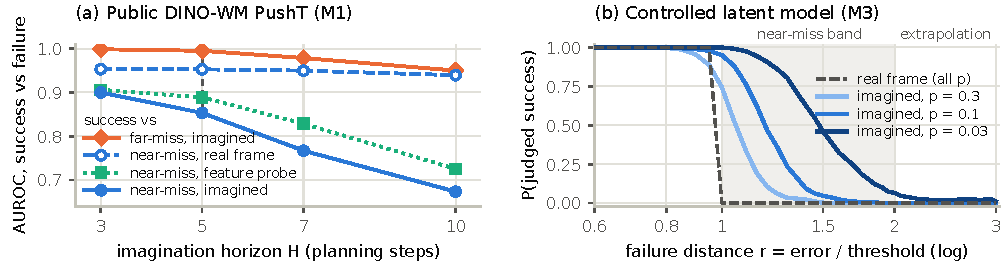
\includegraphics[width=0.85\linewidth]{fig_boundary.pdf}\par
\captionof{figure}{경계 해상도. (a) M1, val 분할, 원 정의 $r$, 판정기 (a). 세로 파선은 사전등록 칸이다. (b) M3, 고정 판정기, seed 3개를 합침. 학습 실패는 $1\le r<2$만 덮는다.}\label{fig:boundary}\par}
\smallskip

\subsection{Experiments (실험)}
{\centering\footnotesize
\setlength{\tabcolsep}{4pt}
\begin{tabular}{lccc}
\toprule
사전등록 지표(판정기 (a), 주 칸) & M1 PushT, $H=5$ & M2 LIBERO & M3, $p=0.03$ \\
\midrule
near-miss를 성공으로 판정: 실제 $\rightarrow$ 상상 & 0.112 $\rightarrow$ 0.147 & 0.051 $\rightarrow$ 0.298 & 0.000 $\rightarrow$ 0.535 \\
AUROC 하락: 성공 대 near / 성공 대 far & 0.100 / 0.005 & 0.275 / 0.137 & 0.107 / 0.000 \\
H1a(near $\ge 0.3$, far의 3배 이상) / H1b(near 특이적 손실) & 불성립 / 성립 & 불성립 / 불성립 & 성립 / 3조항 중 2개 \\
H3: near-miss 오판의 상상 몫 $>0.5$ & 0.24, 불성립 & 0.83, 성립 & 1.00, 성립 \\
H2a: Spearman$(n_\pi, o^{\rm imag}_\pi)\ge 0.6$ & 0.36, 불성립 & 하지 않음 & 0.83, 성립 \\
\bottomrule
\end{tabular}\par
\captionof{table}{사전등록 판정. 1차 가설 H1a, H1b, H2a는 각각 한 모델에서만 성립해 ``모델 2개 이상'' 규칙을 채우지 못한다. 탐색 가설 H3은 M2(판정기 단서 있음)와 M3에서 성립한다.}\label{tab:tests}\par}
\smallskip

\textbf{공개 latent 모델의 경계 손실(M1).} $H=5$에서 성공 대 near-miss AUROC는 0.100 [95\% CI 0.075, 0.125] 떨어지고, 성공 대 far-miss AUROC는 0.005 [0.001, 0.010]만 떨어진다. near-miss 쪽 하락은 $H$ 1단위마다 0.031 [0.025, 0.039]씩 커진다(그림~\ref{fig:boundary}a). 특이성에는 한계가 있다. $H=5$를 넘으면 far-miss도 흐려지고(0.021, 0.048), 물체 자세 오차 정의에서는 모든 $H$에서 흐려진다(0.058--0.129). 상상 특징 판별기는 0.889에 그친다(하락 0.064 [0.046, 0.084]). 손실의 일부는 정보 자체에 있다. 오판은 양방향이다. 성공을 성공으로 보는 비율은 줄고(0.862에서 0.710) near-miss를 성공으로 보는 비율은 는다(0.112에서 0.147).
\textbf{성공 편중 데이터가 흐림을 낙관으로 바꾼다(M3, 탐색 가설 H4a).} $p$를 0.3, 0.1, 0.03으로 낮추면 near-miss 오판은 0.10, 0.24, 0.54로 늘고 성공 오판은 0.021, 0.005, 0.000으로 준다($p=0.03$ 대 0.3: $+0.431$ [0.406, 0.457], $-0.021$ [$-0.030$, $-0.014$]; 그림~\ref{fig:boundary}b). 실제 프레임 판정이 완벽하고 상상 특징 판별기도 0.986에 이르므로, 이 오판은 정보 손실보다는 주로 성공 쪽으로 밀린 것이다. 상상이 더한 과대 추정은 near-miss 비중을 따른다(비중을 분석 전에 정한 $1\le r<1.2$로 재면 Spearman 0.83 [0.77, 0.94], $1\le r<2$로 재면 0.66). 실제 성공률이 0.48--0.53인 정책들이 상상에서 0.58, 0.72, 0.99로 갈리지만 순서는 그대로다. M1은 부분 결과다. 짧은(3,000 step) 성공 편중 미세조정은 성공 오판만 줄였고(near-miss 오판 증가는 물체 자세 정의에서만 나타났다), checkpoint 24개의 $o^{\rm imag}_\pi$는 $-0.01$부터 $+0.06$ 사이에 머문다.
\textbf{처방(탐색).} 노출량을 맞추면 경계 겨냥 반사실은 재가중을 한 번도 이기지 못했다(설정 3개 중 0개, M3에서는 0.040과 0.046만큼 나쁨). 그래서 처방으로 제안하지 않는다. M1에서 MC dropout 할인은 정책 편향의 평균 절댓값을 0.0233에서 0.0187로($-0.0046$ [$-0.0088$, $-0.0004$]), 실패 기하 가중 순위 오류를 0.0225에서 0.0171로 줄인다. M1의 편향 자체가 작아 이득도 작다.
\textbf{비디오 월드모델.} M2에서는 near-miss와 함께 far-miss도 흐려진다(경계 특이적 양상 없음). near-miss 오판의 대부분을 상상이 더하지만(0.051에서 0.298), 실제 프레임으로 학습한 판정기가 상상 프레임에서 운영점이 흔들리므로 이 몫의 일부는 판정기에서 왔을 수 있다. \textbf{용량}(사전등록 밖): M3의 near-miss 오판은 예측기가 작을 때 1.000, 기본일 때 0.535, 클 때 0.149다.

\par\vspace{1pt}\noindent{\scriptsize\textbf{참고문헌.}
[1]~G.~Zhou, H.~Pan, Y.~LeCun, L.~Pinto, DINO-WM, arXiv:2411.04983, 2024.
[2]~M.~J.~Kim et al., Cosmos Policy, arXiv:2601.16163, 2026.
[3]~J.~Xu et al., CureWM, arXiv:2610.09134, 2026.
[4]~T.~Yang et al., MiraBench, arXiv:2605.29360, 2026.
[5]~B.~Liu et al., LIBERO, NeurIPS Datasets and Benchmarks, 2023.
[6]~C.~Chi et al., Diffusion Policy, RSS, 2023.\par}

\end{mdframed}

\end{document}
